\documentclass{article}
\usepackage{kotex}

\usepackage{array}
\usepackage{caption}
\usepackage{fancyhdr}
\usepackage{atbegshi}
\usepackage{hyperref}
\usepackage{listings}
\usepackage{etoolbox}
\usepackage{setspace}
\usepackage{color}
\usepackage{graphicx}
\usepackage[
    type={CC},
    modifier={by},
    version={4.0},
]{doclicense}

\definecolor{light-gray}{gray}{0.95}
\definecolor{gray}{gray}{0.4}
\lstset{
    columns=fullflexible,
    frame=tlbr,
    extendedchars=false,
    inputencoding=utf8,
    backgroundcolor=\color{light-gray},
    xleftmargin=0.5cm,
    framesep=4pt,
    framerule=0pt
}

\AtBeginEnvironment{quote}{\par\singlespacing}

\fancyhf{}
\pagestyle{fancy}

\title{Introduction to C Programming Language}
\author{서영원}
\date{April 2024}
\begin{document}



\maketitle

\tableofcontents

\vfill
\doclicenseThis


\pagebreak

\section{사전 준비}

C언어를 사용하기 위해선 \textit{컴파일러}라는 것이 필요하다.
지금은 이해하지 않아도 좋다. 일단 설치해놓자.

\subsection{Windows}

\begin{enumerate}
    \item \url{https://www.msys2.org/}에서 최신버전 msys2를 설치한다.
    \item msys2를 실행하고 `pacman -S mingw-w64-ucrt-x86\_64-gcc'를 입력한다.
    \item `Proceed with installation? (Y/n)'이 출력되면 엔터키를 입력한다.
    \item 제대로 설치되었는지 확인하기 위해 `gcc --version'을 입력한다.
    \item 제대로 설치되었다면, `gcc.exe 어쩌고 저쩌고...'등이 출력될 것이다.
\end{enumerate}

앞으로, gcc를 실행하라는 문장이 본문에서 발견되면, msys2를 실행하고 명령어를 입력하도록 하자.

\subsection{Linux}

리눅스 사용자라면, 자신의 패키지관리자가 무엇인지 알고 있을 것이다.
해당 패키지관리자에서 \textit{gcc}를 설치하도록 하자.

\section{C언어의 탄생}

운영체제와 브라우저, 온갖 응용프로그램들까지 현대에 이르러 더이상
C언어의 손길을 거치지 않은 프로그램은 없다.
컴퓨터는 인간이 이해할 수 있는 언어는 이해하지 못한다고들 하는데,
그렇다면 C언어는 어떻게 컴퓨터 시스템에서 실행될 수 있을까?
인간이 지금껏 사용해온 언어, 자연어는 왜 컴퓨터 시스템에서 사용되지 않는
것일까?

\subsection{자연어의 모호성}

\begin{quote}
`마트가서 우유사고 만약에 아보카도 있으면 6개 사와'
\end{quote}

오늘 독자가 아내로부터 하달받은 명령이다.
우리는 이를 해석함에 있어서 다음과 같이 2가지 해석을 마련할 수 있다.

\begin{center}

    \centering

    아보카도 명령 코드

    \begin{minipage}{0.45\textwidth}
        \begin{lstlisting}[escapeinside=``]
`마트로 이동한다.`
`우유 1개 구매한다.`
`만약 아보카도가 진열되어있다면:`
    `아보카도 6개 구매한다.`
        \end{lstlisting}
    \end{minipage}
    \hfill
    \begin{minipage}{0.45\textwidth}
        \begin{lstlisting}[escapeinside=``]
`마트로 이동한다.`
`만약 아보카도가 진열되어있다면:`
    `우유 6개 구매한다.`
`아니라면:`
    `우유 1개 구매한다.`
        \end{lstlisting}
    \end{minipage}

\end{center}

만에 하나 둘 중에 잘못된 선택지를 골랐다면 (우유 6팩을 구매한다는 둥)
감히 끔찍한 일이 닥치고 말 것이다.

마찬가지로, 컴퓨터를 프로그램함\footnote{프로그램을 컴퓨터에 내장하는 \\
행위}에 있어서 이러한 모호성이 존재할 경우 이가 실행될 때에 컴퓨터는 둘
중 어떠한 행위를 해야할 지 선택해야만 한다. 이는 사용자가 의도하지 않은
동작을 초래할 수 있는 매우 위험한 상태다. 따라서, 그 자체로 모호성을
내재한 자연어는 컴퓨터를 프로그램하기 위한 언어로 적절하지 못하다.

\subsection{명령집합과 기계어}

\begin{table}[!h]
    \centering

    \caption{아보카도 명령 집합}
    \label{Tab:avocado-isa}

    \begin{tabular}{ || m{2em} | m{3.8em} | m{22em} || }
        \hline
        이름 & 매개변수 & 동작 \\
        \hline\hline
        buy & 물품 t, 자연수 n & t를 n개 만큼 구매한다. 아니라면 0으로 정의한다 \\
        \hline
        find & 물품 t & 물품 t가 존재한다면 r을 1로 정의한다. 아니라면 r을 0으로 정의한다. \\
        \hline
        move & 위치 p & r이 0이라면 위치 p로 이동한다. 아니라면 아무 동작도 하지 않는다. \\
        \hline
    \end{tabular}
    \newline
    \textit{\color{gray} \small r은 미지수 내지 변수라고 정의하자.
    아직 너무 엄밀해질 필요는 없다.}
\end{table}

대신, 컴퓨터는 인위적으로 정의된 명령 집합에 따라 작동한다. 아보카도와
우유를 향한 임무 달성을 위해 Table \ref{Tab:avocado-isa} 과 같이 명령
집합을 정의해보자.

이러한 명령집합을 사용하면 아래와 같이 \textbf{엄밀하게} 우리의 행위를
정의해볼 수 있다. (명령은 위에서부터 순차적으로 실행한다.)

\begin{center}

    \centering

    아보카도 명령 코드 (최종)

    \begin{minipage}{0.45\textwidth}
        \begin{lstlisting}[escapeinside=``]
buy(`우유`, 1)
find(`아보카도`)
move(`출구`)
buy(`아보카도`, 6)
        \end{lstlisting}
    \end{minipage}
    \hfill
    \begin{minipage}{0.45\textwidth}
        \begin{lstlisting}[escapeinside=``]
buy(`우유`, 1)
find(`아보카도`)
move(`출구`)
buy(`우유`, 5)
        \end{lstlisting}
    \end{minipage}

\end{center}

이렇게만 적어도 사람이 프로그램을 수행함에 있어서 어려움은 없다.
그러나, 전류 흐름의 여부로 신호를 처리하는 컴퓨터에게 있어서,
한글과 알파벳을 이해하도록 하는 것은 매우 복잡할 것이다.
(컴퓨터가 어떻게 글자를 처리하는 지에 대해선 뒤
\autoref{sec:code-page}와 \autoref{sec:fonts}를 참조하라)

따라서, 우리는 다음과 같이 각각의 명령과 단어들에 번호를 부여할 것이다.

\begin{table}[!h]
    \centering

    \caption{아보카도 명령 집합 (최종)}
    \label{Tab:avocado-isa-int}

    \begin{tabular}{ || c | c | c | c || }
        \hline
        이름 & 번호 & 이름     & 번호 \\
        \hline\hline
        buy  & 0    & 아보카도 & 0    \\
        \hline
        find & 1    & 우유     & 1    \\
        \hline
        move & 2    & 출구     & 2    \\
        \hline
    \end{tabular}
\end{table}

부여된 번호를 통해 다시 구현하면 다음과 같다.

\begin{center}

    \centering

    아보카도 명령 코드 (진짜최종)

    \begin{minipage}{0.45\textwidth}
        \begin{lstlisting}
0(1, 1)
1(0)
2(2)
0(0, 6)
        \end{lstlisting}
    \end{minipage}
    \hfill
    \begin{minipage}{0.45\textwidth}
        \begin{lstlisting}
0(1, 1)
1(0)
2(2)
0(1, 5)
        \end{lstlisting}
    \end{minipage}

\end{center}

또한 다음의 규칙에 따라 명령을 기계가 이해하기 쉽도록 바꾸어보자.

\begin{itemize}
    \item 명령과 상품에는 각각 2비트를 할당하자
    \item 상품의 갯수에는 4비트를 할당하자
\end{itemize}

결과는 다음과 같다:

\begin{center}

    \centering
    
    아보카도 명령 코드 (진짜최종2)

    \begin{minipage}{0.45\textwidth}
        \begin{lstlisting}
00 01 0001
01 00
10 10
00 00 0110
        \end{lstlisting}
    \end{minipage}
    \hfill
    \begin{minipage}{0.45\textwidth}
        \begin{lstlisting}
00 01 0001
01 00
10 10
00 01 0101
        \end{lstlisting}
    \end{minipage}

\end{center}

축하한다! 독자는 방금 마트에 가서 우유 (혹은 아보카도)를 구매할
로봇가정부를 위한 명령 체계\footnote{ISA : Instruction Set Architecture}
를 완성했다!
이제 독자는 독자의 아내에게 \textbf{모호하지 않은} 명령을 내려달라고
요구할 수 있게 되었고, 독자의 아내가 독자에게 부여한 업무를 독자의
로봇에게 \textbf{모호함} 없이 전달할 수 있을 것이다!

\subsection{기계어와 C언어}

...그래서 이 기계어가 C언어랑 무슨 상관일까?
그것은 C언어의 태생에 있다.
자세히 알아보기 위해 1951년으로 돌아가보자.

\subsubsection{복잡해지는 ISA와 어셈블리어}

| 컴퓨터를 프로그램하기 위해 0과 1만 두드리고 있는 것은
매우 지루한 일일 뿐더러, 코드에 오류가 존재하거나 오타를 치고 말았을때
수정하기 매우 번거롭다.

개발자들은 이러한 문제를 해결하기 위해
\textit{어셈블리어}\footnote{ASM : ASseMbly language}
\footnote{
    Maurice Wilkes, David Wheeler와 Stanley Gill의 저서
    \textit{The Preparation of Programs for an Electronic Digital Computer}
    에서 최초로 제시되었다.
    본 도서에는 이 외에 최초로 \textit{재사용 가능한} 코드, \textit{API},
    디버깅을 위해 \textit{메모리 덤프}를 사용하는 방법이 서술되었다.
}를 도입했다. 

이는 독자가 설계한 `아보카도 명령 코드 (최종)'과 비슷한 것으로,
기계어에 일대일 대응되도록 알파벳으로 이루어진 이름을 부여한 것이다.

다음의 규칙과 함께 아래의 명령을 해석해보자:

\begin{table}[!h]
    \centering

    \caption{계산기 ISA}
    \label{Tab:simple-calculator-isa}

    \begin{tabular}{ || m{2em} | m{5em} | m{22em} || }
        \hline
        이름 & 매개변수 & 동작 \\
        \hline\hline
        add  & 값 t & 변수 a에 t만큼 더한 값을 a로 정의한다 \\
        \hline
        mul  & 값 t & 변수 a와 t를 곱한 값을 a로 정의한다 \\
        \hline
        div  & 값 t & 변수 a를 t로 나눈 값을 a로 정의한다 \\
        \hline
        mov  & 변수 a, 값 v & a에 v를 대입한다 \\
        \hline
    \end{tabular}
\end{table}

\begin{center}

    \centering
    
    Table \ref{Tab:simple-calculator-isa}를 이용한 코드

\begin{lstlisting}
mov b, a
add 1
mul b
div 2
mov b, a
\end{lstlisting}
\end{center}

위의 코드는 정의된 ISA에 따라 아래와 같은 수식으로 해석할 수 있다:

\begin{equation}
b = \frac{a(a + 1)}{2}
\end{equation}

하지만, 세상에 이렇게 간단한 코드만 존재했다면 세상은 지금까지조차 ASM을
쓰고 있을지도 모르겠다.
그럼 그렇지, 요즘 많이 사용되는 x86-64 구조는 명령어 약 3,600개 가량을
가지고 있다.
이 것들을 아무런 도움도 없이 활용하여 성능 좋고 보기도 좋은 프로그램을
만드는 것은 매우 어려운 일이다.

\subsubsection{고수준 언어의 등장}

| 개발자들은 \textbf{사람이 이해하기 쉬운} 프로그래밍 언어를 원했다.
결국 1953년, IBM의 John Backus는 세계 최초의 고수준 프로그래밍 언어,
\textit{Speedcoding}을 개발했다.

\begin{figure}[!h]
    \centering
    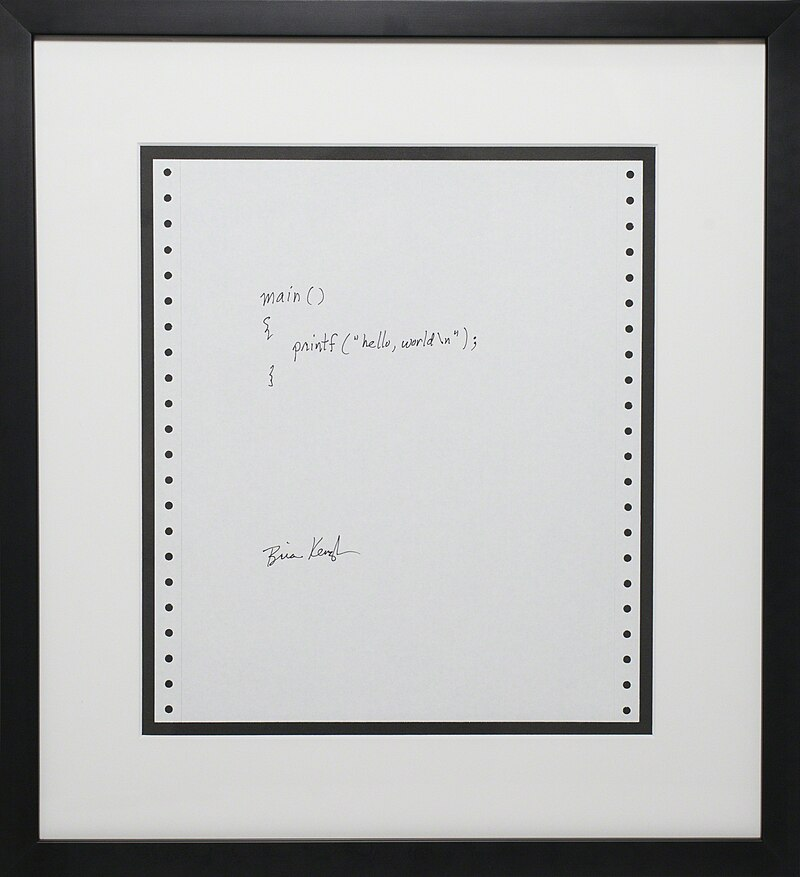
\includegraphics[width=\linewidth]{images/hello-world.jpg}
    \caption{1978년, C언어를 공동개발한 Brian Kernighan의 Hello, World}
\end{figure}

이후 \textit{Fortran}(1957), \textit{ALGOL}(1960), \textit{CPL}(1963)과
\textit{B}(1969)를 거치고, 드디어 1972년 벨 연구소, Dennis Ritchie는
\textit{C}를 개발한다.

\pagebreak

\section{Hello, World!}

C언어는 기본적으로 ASM과 같은 저급언어
\footnote{
    사전적 정의에 따르면, 컴퓨터가 이해하기 쉽게 작성된 프로그래밍 언어라면 모두 저급언어이나, 
    통상적으로 기계어와 ASM만을 가리킨다.
}
을 추상화하기 위해 태어난 여러 언어들의 문제점들을 해결하기 위해 만들어졌다.
따라서, C언어의 문법을 이해하기 위해, 아래 BASIC으로 작성된 예제
\footnote{
    BASIC의 문법은 대체로 Microsoft QuickBASIC의 문법을 차용하였으나,
    독자의 이해를 돕기 위해, 그때 그때 가장 직관적으로 간단해 보이는 문법을 차용하였다.
}
를 살펴보자.
(대부분의 언어들이 Fortran 혹은 Basic과 비슷한 형상을 띄므로)

\subsection{Hello, BASIC!}

\begin{lstlisting}
10 PRINT "Hello, BASIC!"
20 END
\end{lstlisting}

위는 BASIC을 통해 화면에 `Hello, BASIC!'라는 문장을 출력하는 예제다.

영어를 할줄 안다면 대충 이해했을텐데, 
첫 줄의 `PRINT ``Hello, BASIC!"'는 `Hello, BASIC!'라는 문장을 출력하도록 하는 명령,
두번째 줄의 `END'는 프로그램이 종료되었음을 알리는 명령이다.

더 복잡한 예시를 살펴보자.

\begin{lstlisting}
10 N=100
20 FOR I=1 TO N
30 PRINT "Hello, BASIC!"
40 NEXT I
\end{lstlisting}

위의 예시는 다음의 과정에 따라 `Hello, BASIC!'라는 문장을 100번 출력하는 예제다:

\begin{enumerate}
    \item `N=10'은 변수 N의 값을 100으로 정의한다.
    \item `FOR I=1 TO N'은 변수 I를 1로 정의한다.
    `NEXT I'가 호출되었을때, 변수 I의 값을 1 증가시키고,
    I가 N 이하라면 `FOR I=1 TO N'의 직후로 돌아간다.
    \item `PRINT ``Hello, BASIC!"'는 `Hello, BASIC!'라는 문장을 출력한다.
    \item `NEXT I'는 I가 N이하인 동안 `FOR I=1 TO N'부터 `NEXT I'까지의 명령들이 반복해서 실행되도록 한다.
\end{enumerate}

물론, 입력도 받지 않고 출력만 하는 프로그램은 쓸모가 없다.
다음의 예시를 살펴보자:

\begin{lstlisting}
10 INPUT "How many stars? "; C
20 S$ = ""
30 FOR I=1 TO C
40 S$ = S$ + "*"
50 NEXT I
60 PRINT S$
70 INPUT "Do you want more? "; A$
80 IF LEN(A$) = 0 THEN GOTO 70
90 IF A$ = "y" OR A$ = "Y" THEN GOTO 10
100 PRINT "Goodbye"
110 END
\end{lstlisting}

\begin{enumerate}
    \item `INPUT ``How many stars? "; C' : `How many stars? '를 출력하고, 숫자를 변수 C를 입력받는다.
    \item `S\$ = ``"' : 문자열 변수 S\$의 값을 빈 문자열(`')로 정의한다.
    \item `FOR I=1 TO C' : I를 1부터 C까지 반복한다.
    \item `S\$ = S\$ + ``*"' : 문자열 S\$에 `*'를 덧붙인다.
    \item `NEXT I' : I가 C 이하라면 30번째 명령으로 돌아간다.
    \item `PRINT S\$' : 문자열 S\$를 출력한다.
    \item `INPUT ``Do you want more? "; A\$' : `Do you want more? '을 출력하고, 문자열을 변수 A\$에 입력받는다.
    \item `IF A\$ = ``y" OR A\$ = ``Y" THEN GOTO 10' : 만약 A\$가 `y'거나 `Y'라면 10번 명령으로 이동한다.
    \item `PRINT ``Goodbye"' : `Goodbye'를 출력한다.
    \item `END' : 프로그램을 종료한다
\end{enumerate}

결국, 위 프로그램은 입력받은 숫자만큼 `*'을 출력하는 프로그램이다.

프로그래밍에 익숙하지 않거나, `goto'를 사용해본적 없다면, 위 코드부터 슬슬 어지러움을 느낄 수 있다.
물론, 아직까지 어지럼증을 느끼지 않을 순 있으나, `*'와 `-' 중 선택한 문자를 출력하도록 하는 프로그램이라던지,
여러 기능들을 추가하다보면 점점 내가 뭘 하고있는지 알수 없게되는 시점이 온다.

이를 해결하기 위해 개발자들은 언어를 `구조화'시키기 시작했다.

\subsection{언어의 구조화}

\subsubsection{Label과 Goto}

개발자는 먼저 줄번호(명령의 앞에 붙어 명령의 번호와 순서를 지정하는 번호)를 없애고, 대신 `레이블(label)'을 도입했다.
예를 들면 다음과 같다:

\begin{center}

    \centering
    
    줄번호를 이용한 BASIC(좌)과 label을 이용한 BASIC(우)

    \begin{minipage}{0.45\textwidth}
        \begin{lstlisting}
10 PRINT "Hello!"
20 GOTO 10
        \end{lstlisting}
    \end{minipage}
    \hfill
    \begin{minipage}{0.45\textwidth}
        \begin{lstlisting}
Print:
PRINT "Hello!"
GOTO Print
        \end{lstlisting}
    \end{minipage}

\end{center}

훨씬 가독성이 좋아진 모습이나,
`GOTO'가 코드에 보이는 것 조차 싫었던 개발자들은 `GOTO'없이 코드를 작성하기 위해 여러 문법 설탕
\footnote{
    Syntax Sugar, Syntactic Sugar.
    없으면 프로그램을 구현하지 못하는게 아닌데도, 즉, 컴퓨터가 아니라 사람이 이해하고 표현하기 쉽게 설계된 문법.
}
들과 `서브루틴(subroutine)'의 개념을 추가했다.

\subsubsection{DO WHILE ... LOOP}

2세대 BASIC언어들에는 참 많은 문법 설탕들이 있지만, 그중에서도 `DO WHILE ... LOOP'를 소개하고자 한다.



`GOTO'를 이용한 BASIC(상)과 `DO WHILE ... LOOP'를 이용한 BASIC(하)

\begin{lstlisting}
Print:
PRINT "Hello, BASIC!"
INPUT "Want one more line? "; S$
IF S$ = "y" OR S$ = "Y" THEN GOTO Print
\end{lstlisting}
\begin{lstlisting}
PRINT "Hello, BASIC!"
INPUT "Want one more line? "; S$
DO WHILE S$ = "y" OR S$ = "Y"
    PRINT "Hello, BASIC!"
    INPUT "Want one more line? "; S$
LOOP
\end{lstlisting}

label을 없애고 WHILE을 통해 직관적으로 반복문의 구조와 조건을 밝히며 가독성을 높이고 있다.
그러나, 같은 명령이 두번씩 반복되는 것은 그다지 좋지 않은 코드
\footnote{
    코드의 재사용성을 낮춘다. 같은 기능을 하는 명령들을 전체 코드 곳곳에 복붙해두었는데,
    몇달이 지나고 기능을 변경해야한다고 생각해보자.
    복붙해둔 모든 곳을 찾아다니며 코드를 변경해야한다!
}
다. 

이런 상황을 위해 `DO ... LOOP WHILE'문이 준비되어있다.



`DO WHILE ... LOOP'를 이용한 BASIC(상)과 `DO ... LOOP WHILE'을 이용한 BASIC(하)

\begin{lstlisting}
PRINT "Hello, BASIC!"
INPUT "Want one more line? "; S$
DO WHILE S$ = "y" OR S$ = "Y"
    PRINT "Hello, BASIC!"
    INPUT "Want one more line? "; S$
LOOP
\end{lstlisting}
\begin{lstlisting}
S$ = ""
DO
    PRINT "Hello, BASIC!"
    INPUT "Want one more line? "; S$
LOOP WHILE S$ = "y" OR S$ = "Y"
\end{lstlisting}


반복문 내의 코드를 실행하기 이전에 조건을 검사해, 두번씩 작성되던 코드를 한번만 작성할 수 있게 했다.

이와 같이 BASIC과 많은 언어들은 문법 설탕을 첨가하며 발전해왔고, C언어 또한 이러한 구조들을 채택하고 있다.
이제 서브루틴에 대해 알아보자.



\subsubsection{서브루틴}

특정한 갯수 만큼 별표(`*')를 출력하는 등 자주 반복되는 명령들을 하나로 묶어서 사용할 순 없을까?
묶어서 사용할 수만 있으면, 같은 명령어들이 반복해서 쓰이는 상황들도 효과적으로 줄일 수 있을 것이다.

이러한 고민 속에 탄생한 것이 서브루틴으로,
단순히 말하자면, 특정한 일을 처리하기 위해 일련의 명령어들을 묶어둔 것이다.

쉬운 이해를 위해 BASIC코드를 보며 이해해보자:

\begin{lstlisting}
10 GOSUB 100
20 PRINT "Bye, SUBROUTINE!"
30 END
100 PRINT "Hello, SUBROUTINE!"
110 RETURN
\end{lstlisting}

위 코드에서 `GOSUB 100'은 `GOTO'와 같이 줄번호 100으로 점프하고,
`PRINT ``Hello, SUBROUTINE!"'과 `RETURN'을 순차적으로 실행시킨다.
유일한 차이점은, `RETURN'이 실행되면 줄번호 10의 자리로 돌아와
'PRINT ``Bye, SUBROUTINE!"을 실행한다는 것이다.

이와 같이 서브루틴은 특정한 주소 공간에 명령어를 모아서 작성할 수 있게 하고,
이를 통해 코드의 유지보수를 쉽게 만들어준다.

그러나, 기술이 발전하고 BASIC에서 줄번호를 없애는 과정속에서 `GOSUB' 또한 개량되어야 했다.
이를 해결하기 위해 개발자들은 `함수(function)'이라는 개념을 도입했다.

\subsubsection{함수}

독자가 한국인이라면, 함수는 중학교에서 알게된 수학 용어일 것이다.
프로그래밍에서의 `함수'또한 비슷한 의미로,
입력을 받아 (정의역에 대해) 일을 처리하기 위해 (출력을 가지기 위해; 치역을 가지기 위해)
묶어놓은 일련의 명령어 묶음
\footnote{
    함수형 프로그래밍을 사랑하는 개발자분들은 화내지 말아주길 바란다.
    이는 어디까지나 BASIC이나 C를 기준으로 작성된 것으로,
    독자의 이해를 쉽게하기 위해 `프로그래밍에서의 함수'로 성급하게 일반화된 것이다.
}
이다. (물론, 입력을 받지 않아도 좋다. 이에 대해선 후술한다.)

BASIC에서는 함수를 다음과 같이 작성한다:

\begin{lstlisting}[escapeinside=``]
SUB `함수명`(`매개변수1`, `매개변수2`, ...)
    `명령어...`
END SUB
\end{lstlisting}

위에서 `GOSUB'와 함께 서술된 코드를 함수 문법을 통해 다시 작성해보자:

\begin{lstlisting}
CALL PrintHello()
PRINT "Bye, SUBROUTINE!"
END

SUB PrintHello()
    PRINT "Hello, SUBROUTINE!"
END SUB
\end{lstlisting}

위와 같이, 그저 반복되는 명령어들을 하나로 함축하기 위함이라면 매개변수,
즉 입력을 받지 않아도 좋다.

\subsection{Hello, C!}

C언어는 상술된 개념들을 대부분 문법적인 개량만 가지고 차용하고 있다.
이제 C언어를 통해 `Hello, World!'를 출력해보자!


\begin{lstlisting}
main()
{
    printf("Hello, World!\n");
}
\end{lstlisting}

위 코드를 `main.c'파일에 저장하고, 다음의 명령어를 실행해 실행파일
\footnote{
    Unix계열이라면 a.out, Windows라면 a.exe가 기본 출력파일명이다.
}
을 만들어보자.

\begin{lstlisting}[language=bash]
$ ls
main.c
$ gcc main.c
$ ls
a.out main.c
$ ./a.out
Hello, World!
\end{lstlisting}

먼저, 터미널(Windows라면 msys2)을 열고,
`main.c'가 존재하는 폴더까지 이동한다.
그 후, `gcc main.c'를 입력해 `main.c'로부터 실행파일을 생성하도록 하자.

이제, 위의 C언어 코드를 분석해보자.
위 C언어 코드는 아래의 BASIC 코드와 동일하다:

\begin{lstlisting}
CALL main()

SUB main()
    PRINT "Hello, World!"
END SUB
\end{lstlisting}

C언어에서는 함수를 정의하는데에 있어서,
서브루틴이라는 개념보다 본격적으로 수학에서의 함수를 닮았다.

수학에서 함수를 $f(x) = ...$와 같이 서술했던 것과 비슷하게,
C언어에서도 함수를 $f(x) { ... }$라고 작성한다.
물론, 입력을 받지 않고 단순하게 $f()$라고도 작성할 수 있다.

비슷한 맥락에서, $main()$은 매개변수를 가지지 않는 `main'이라는 이름의 함수를 선언한 것이고,
그 밑의 ${ ... }$는 이 함수가 어떤 일을 하는지 서술한다.

따라서, 위의 C언어 코드의 $main()$은 호출되었을때,
`Hello, World!\\n'
/footnote{
    `\\n'은 개행을 표현하는 이스케이프 문자(Escape Character)로,
    소스코드에서 표현하기 어려운 문자들
    (개행문자(line-break character), 탭 문자(tab character, tabulator character) 등)
    을 표현하기 위해 `\\'와 특정한 문자를 결합해 대신 사용할 수 있도록 설계된 것이다.
}
를 출력하는 함수라고 말할 수 있다.

또한, BASIC에서만 볼 수 있는 첫 행의 `CALL main()'은 왜 추가된 것일까?
사실, C언어에서는 BASIC처럼 함수에 포함되지 않는 명령을 작성할 수 없다.
글로 읽어서는 이해하기 힘든데, 다음의 코드를 보며 이해해보자:

\begin{center}

    \centering
    
    문법적인 오류가 있는 코드(좌)와 올바른 코드(우)

    \begin{minipage}{0.45\textwidth}
        \begin{lstlisting}
printf("Hello, World!");
printf("Bye...");
        \end{lstlisting}
    \end{minipage}
    \hfill
    \begin{minipage}{0.45\textwidth}
        \begin{lstlisting}
main()
{
    printf("Hello, World!");
    printf("Bye...");
}
        \end{lstlisting}
    \end{minipage}

\end{center}

위와 같이, 모든 명령은 함수 내부에 있어야 한다.

또한, 유독 $main()$이라는 이름이 많이 보이는 것 같다면 착각이 아니다.
프로그램의 진입점, 즉 프로그램이 시작하는 부분을 BASIC에서는 위에서부터 순차적으로 실행했다면,
C언어에서는 $main()$라는 함수를 진입점으로 사용하여, $main()$ 함수 내부의 명령부터 실행하게 된다.

\subsubsection{세미콜론;;;}

C 코드를 보다보면, 눈에 띄는 기호 하나가 보인다.
바로 세미콜론(;)인데, BASIC에서 명령과 명령을 개행으로 구분했다면,
C언어에서는 이 세미콜론으로 명령을 구분하기 때문에,
모든 명령의 끝에는 세미콜론이 자리잡고 있다.

왜 개행이 아닌 세미콜론을 사용했는지,
세미콜론을 사용해서 얻은 이점이 뭔지에 대해선 \autoref{sec:code-beauty}에서 서술하도록 하겠다.

\section{변수와 printf}

\appendix

\section{세미콜론의 아름다움}
\label{sec:code-beauty}

\section{글자의 순번, Code Page}
\label{sec:code-page}

\section{글자의 형태, Font}
\label{sec:fonts}

\section{CISC와 RISC}
\label{sec:cisc-risc}

\end{document}